\section{Experiments}

I decided to do perform two kinds of experiments: the first is devoted to find relationships between the number of frequent items the algorithm is able to find, the threshold and the execution time. My thesis was: the higher the threshold, the faster the algorithm will finish but the less number of results will be found. This is not surprising at all: if we increment the threshold we are asking to a generic k-tuple of elements, in order to be considered frequent, to appear a number of times which is higher and higher. With this experiment I wanted to check how fast this reduction would happen, i was expecting a gradual lowering of the frequent set cardinality, the result denies me:
\begin{figure}[h]
    \caption{Relationships between execution time, support threshold, number of frequent items found}
    \centering
    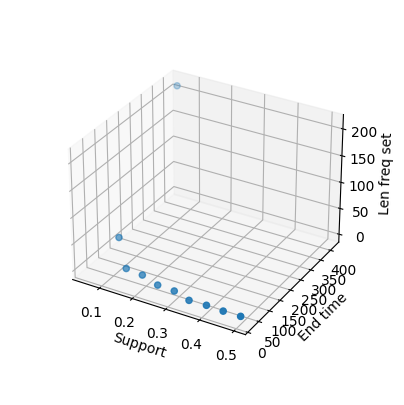
\includegraphics[width=0.5\textwidth]{project_report_src/project_report_images/support_end-time_len-freq-set.png}
\end{figure}

when the threshold changes from the 5\% to the 10\% the number of frequent items decreases abruptly: 211 with the first threshold and 48 with the latter.This result means that there a lot of k-tuples which are somehow borderline: they are frequent with the first threshold but the number of occurencies is very close to the threshold itself. This may be related to the fact that the structure of language is very complex, for example the presence of synonyms can lead to this result. In fact, there are a lot of words which can be used instead of "good", for example, and those words are used by a smaller number of reviewers, for this reason the itemsets with "delicious" (for example) as item are took into consideration with $threshold = 0.05$ but not with $threshold = 0.10$ . As I suspected the execution time got lower as the threshold increased, this is a natural behaviour given by the structure of the algorithm: when the threshold increases it is able to filter out more elements and this filtering allows to create less k-tuples, for this reason the overall computational time get lower.

The second experiment had the aim of checking the scaling for the algorithm. I runned the algorithm with an incremental number of rows from $1 \cdot 10^5$ to $7 \cdot 10^5$, with $1 \cdot 10^6$ and with $1.5 \cdot 10^6$ and i checked only the execution time:
\begin{figure}[h]
    \caption{Relationships between execution time and number of rows}
    \centering
    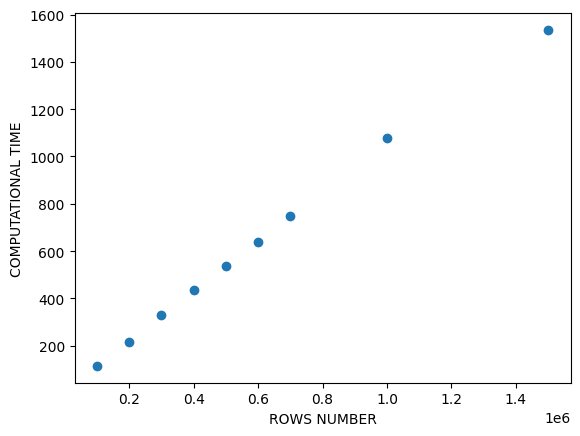
\includegraphics[width=0.5\textwidth]{project_report_src/project_report_images/scaling.png}
\end{figure}
the growth is linear, this is a good signal for the algorithm robustness. 